\documentclass[12pt,letterpaper]{SANDreport}

\usepackage{amsthm,amssymb,amsfonts,amsmath}
\usepackage{color}
%\usepackage{pslatex}
\usepackage{mathptmx}	% Use the Postscript Times font
\usepackage[FIGBOTCAP,normal,bf,tight]{subfigure}
\usepackage{multirow}
\usepackage{verbatim}
\usepackage{nicefrac}

%%% ====================================================================
%%% @LaTeX-file{
%%%    filename  = "SANDmath.tex",
%%%    version   = "1.2",
%%%    date      = "2005/01/08",
%%%    author    = "Philippe P. Pebay",
%%%    address   = "Sandia National Laboratories, PO Box 969,
%%%                 MS 9051, Livermore, CA 94550, USA",
%%%    email     = "pppebay@ca.sandia.gov",
%%%    supported = "yes",
%%%    abstract  = "This is a LaTeX documentclass that provides 
%%%                 mathematical environments and macros for Sandia 
%%%                 technical reports (SAND reports).",
%%% }
%%% ====================================================================
\typeout{Using SANDmath LaTeX Package: August 1,
2005, v1.2 Philippe P. Pebay}
% ----------------------------------------------------------------------
% -- Packages
% ----------------------------------------------------------------------
\usepackage{latexsym}
\usepackage{amssymb,amsfonts,amsmath,amsthm}
\usepackage{calrsfs}
\usepackage{stmaryrd}
\usepackage[mathscr]{eucal}
% ----------------------------------------------------------------------
% -- Mathematical environment
% ----------------------------------------------------------------------
% -- equation environment
\numberwithin{equation}{section}
% -- theorems & related topics
\theoremstyle{plain}
\newtheorem{theo}{Theorem}[section]
\newtheorem{prop}[theo]{Proposition}
\newtheorem{lemm}[theo]{Lemma}
\newtheorem{coro}[theo]{Corollary}
% -- definitions & axioms
\theoremstyle{definition}
\newtheorem{defi}{Definition}[section]
\newtheorem{axio}{Axiom}[section]
% -- remarks & examples
\theoremstyle{remark}
\newtheorem{rema}{Remark}[section]
\newtheorem{exam}{Example}[section]
% -- algorithms
\newtheoremstyle{algostyle}% name
  {}%      Space above, empty = `usual value' 
  {}%      Space below
  {\sffamily}%         Body font
  {0pt}%         Indent amount (empty = no indent, \parindent = para indent)
  {\bfseries}% Thm head font
  {}%        Punctuation after thm head
  { }% Space after thm head: \newline = linebreak
  {\thmname{#1}\thmnumber{ \thesection.#2}{ [#3]}}% Thm head spec
\theoremstyle{algostyle}
\newtheorem{algo}{Algorithm}
% ----------------------------------------------------------------------
% -- Mathematical macros
% ----------------------------------------------------------------------
% -- K, N, Z, R & C
\newcommand{\K}{{\rm I\kern-.16em K}}
\newcommand{\N}{{\rm I\kern-.16em N}}
\newcommand{\Z}{\mathchoice{\sf\textstyle Z\kern-0.4em Z}%
{\sf\textstyle Z\kern-0.4em Z}%
{\sf\scriptstyle Z\kern-0.3em Z}%
{\sf\scriptscriptstyle Z\kern-0.2em Z}}%
\newcommand{\R}{{\rm I\kern-.16em R}}
\newcommand{\C}{\mathchoice{\setbox0=\hbox{$\displaystyle\rm C$}%
\hbox{\hbox to0pt{\kern0.4\wd0\vrule height0.9\ht0\hss}\box0}}%
{\setbox0=\hbox{$\textstyle\rm C$}\hbox{\hbox%
to0pt{\kern0.4\wd0\vrule height0.9\ht0\hss}\box0}}%
{\setbox0=\hbox{$\scriptstyle\rm C$}\hbox{\hbox%
to0pt{\kern0.4\wd0\vrule height0.9\ht0\hss}\box0}}%
{\setbox0=\hbox{$\scriptscriptstyle\rm C$}\hbox{\hbox%
to0pt{\kern0.4\wd0\vrule height0.9\ht0\hss}\box0}}}
% -- discrete intervals
\newcommand{\cdi}[2]{\llbracket{#1},{#2}\rrbracket}
\newcommand{\odi}[2]{\rrbracket{#1},{#2}\llbracket}
\newcommand{\codi}[2]{\llbracket{#1},{#2}\llbracket}
\newcommand{\ocdi}[2]{\rrbracket{#1},{#2}\rrbracket}
% -- functional spaces
\newcommand{\CC}[1]{{\mathcal{C}^{#1}}}
\newcommand{\CCs}[2]{{\mathcal{C}^{#1}_{#2}}}
\newcommand{\Lsp}[1]{{\mathrm{L}^{\scriptstyle#1}}}
\newcommand{\Lo}{\Lsp{1}}
\newcommand{\Lt}{\Lsp{2}}
\newcommand{\Li}{\Lsp{\infty}}
% -- differential calculus
\newcommand{\dd}[1]{\mathrm{d}{#1}}
\newcommand{\der}[2]{\frac{\dd{#1}}{\dd{#2}}}
\newcommand{\lder}[2]{\frac{\dd{}}{\dd{#2}}{#1}}
\newcommand{\dern}[3]{\frac{\mathrm{d}^{#1}{#2}}{\dd{#3}^{#1}}}
\newcommand{\ldern}[3]{\frac{\mathrm{d}^{#1}}{\dd{#3}^{#1}}{#2}}
\newcommand{\pder}[2]{\frac{\partial{#1}}{\partial{#2}}}
\newcommand{\lpder}[2]{\frac{\partial}{\partial{#2}}{#1}}
\newcommand{\pdern}[3]{\frac{\partial^{#1}{#2}}{\partial{#3}^{#1}}}
\newcommand{\lpdern}[3]{\frac{\partial^{#1}}{\partial{#3}^{#1}}{#2}}
\newcommand{\pxder}[3]{\frac{\partial^2{#1}}{\partial{#2}\partial{#3}}}
\newcommand{\lpxder}[3]{\frac{\partial^2}{\partial{#2}\partial{#3}}{#1}}
\newcommand{\dive}{\operatorname{div}}
\newcommand{\grad}{\operatorname{grad}}
\newcommand{\curl}{\operatorname{curl}}
\newcommand{\Nd}[1]{\nabla\cdot{#1}}
\newcommand{\Ng}[1]{\nabla\,{#1}}
\newcommand{\Nc}[1]{\nabla\times{#1}}
% -- integral calculus
\newcommand{\sint}[4]{\int_{#1}^{#2}{#3}\,\dd{#4}}
\newcommand{\dint}[3]{\iint_{#1}{#2}\,\dd{#3}}
\newcommand{\ddint}[4]{\iint_{#1}{#2}\,\dd{#3}\dd{#4}}
\newcommand{\tint}[3]{\iiint_{#1}{#2}\,\dd{#3}}
\newcommand{\ttint}[5]{\iiint_{#1}{#2}\,\dd{#3}\dd{#4}\dd{#5}}
% -- vector calculus
\newcommand{\norm}[1]{\left\lVert{#1}\right\rVert}
\newcommand{\normone}[1]{\norm{#1}_1}
\newcommand{\normtwo}[1]{\norm{#1}_2}
\newcommand{\normsup}[1]{\norm{#1}_\infty}
\newcommand{\normgen}[2]{\norm{#2}_{#1}}
\newcommand{\normLo}[1]{\norm{#1}_\Lo}
\newcommand{\normLt}[1]{\norm{#1}_\Lt}
\newcommand{\normLi}[1]{\norm{#1}_\Li}
\newcommand{\normL}[2]{\norm{#2}_\Lsp{#1}}
\newcommand{\seminorm}[2]{\left\lvert{#2}\right\rvert_{#1}}
\newcommand{\indnorm}[1]{\left\lVert\!\left\lvert{#1}\right\rVert\!\right\lvert}
\newcommand{\innprod}[2]{\left({#1}|{#2}\right)}
\newcommand{\dualpair}[2]{\left\langle{#1},{#2}\right\rangle}
\newcommand{\mixprod}[3]{\left[{#1},{#2},{#3}\right]}
% -- asymptotic notations
\newcommand{\smallo}[1]{\operatorname{o}\left({#1}\right)}
\newcommand{\bigo}[1]{\operatorname{O}\left({#1}\right)}
\newcommand{\aseq}[2]{\operatornamewithlimits{\sim}_{{#1}\rightarrow{#2}}}
%%%%%%%%%%%%%%%%%%%%%%%%%%%%%%%%%%%%%%%%%%%%%%%%%%%%%%%%%%%%%%%%%%%%%%%


% If you want to relax some of the SAND98-0730 requirements, use the "relax"
% option. It adds spaces and boldface in the table of contents, and does not
% force the page layout sizes.
% e.g. \documentclass[relax,12pt]{SANDreport}
%
% You can also use the "strict" option, which applies even more of the
% SAND98-0730 guidelines. It gets rid of section numbers which are often
% useful; e.g. \documentclass[strict]{SANDreport}

\newtheoremstyle{example}{\topsep}{\topsep}%
  {}%         Body font
  {\parindent}%         Indent amount (empty = no indent, \parindent = para indent)
  {\bfseries}% Thm head font
  {}%        Punctuation after thm head
  {\newline}%     Space after thm head (\newline = linebreak)
  {\thmname{#1}\thmnumber{ #2}\thmnote{ #3}}%         Thm head spec

\theoremstyle{example}
\newtheorem{example}{Example}[section]

\newcommand{\finish}[1]{\textcolor{red}{\textit{finish}: #1}}
\newcommand{\inner}[2]{\langle #1,#2 \rangle}

% \begin{argtable}{name}{caption}{width}{label}
\newenvironment{argtable}[4]{
   \begin{table}[ht]
     \label{#4}
     \centering
     \caption[#1]{#2}
     \begin{tabular}{|l|l|p{#3}|}
}
{
    \hline
    \end{tabular}
    \end{table}
}

% \at_method{method signature}
\newcommand{\atmethod}[1]{\hline\hline\multicolumn{3}{|l|}{\tt{#1}}\\\hline}

% \at_argument{name}{in/out}{description}
\newcommand{\atargument}[3]{\texttt{#1}&\texttt{#2}&#3\\}

\newcommand{\range}[1]{\mathcal{R}(#1)}


% ---------------------------------------------------------------------------- %
%
% Set the title, author, and date
%
\title{Orthogonalization Study and Design Document for the Anasazi and Belos
Iterative Solver Packages}

\author{Christopher G. Baker \\
Sandia National Laboratories\\
M.S. 1320, P.O. Box 5800\\
Albuquerque, NM 87185-1320 \\
cgbaker@sandia.gov \\
\\
\and
Heidi K. Thornquist \\
Sandia National Laboratories \\
M.S. 0316, P.O. Box 5800\\
Albuquerque, NM 87185-0316 \\
hkthorn@sandia.gov
}

% There is a "Printed" date on the title page of a SAND report, so
% the generic \date should generally be empty.
\date{}


% ---------------------------------------------------------------------------- %
% Set some things we need for SAND reports. These are mandatory
%
\SANDnum{SAND2007-xxxx}
\SANDprintDate{October 2007}
\SANDauthor{Christopher G. Baker, Heidi K. Thornquist}


% ---------------------------------------------------------------------------- %
% Include the markings required for your SAND report. The default is "Unlimited
% Release". You may have to edit the file included here, or create your own
% (see the examples provided).
%
% \include{MarkUR} % Not needed for unlimited release reports



% ---------------------------------------------------------------------------- %
% The following definition does not have a default value and will not
% print anything, if not defined
%
% \SANDsupersed{SAND1901-0001}{January 1901}


% ---------------------------------------------------------------------------- %
%
% Start the document
%
\begin{document}
\maketitle

% ------------------------------------------------------------------------ %
% An Abstract is required for SAND reports
%
\begin{abstract}
  The current framework for orthogonalization in the Anasazi eigensolver package and the
  Belos linear solver package is reviewed. Current orthogonalization needs are described,
  illustrating shortcomings with the current framework, and modifications are proposed.
\end{abstract}



% ------------------------------------------------------------------------ %
% The table of contents and list of figures and tables
% Comment out \listoffigures and \listoftables if there are no
% figures or tables. Make sure this starts on an odd numbered page
%
\cleardoublepage		% TOC needs to start on an odd page
\tableofcontents
%\listoffigures
%\listoftables



% ---------------------------------------------------------------------- %
% An optional glossary. We don't want it to be numbered
% \clearpage
% \section*{Nomenclature}
% \addcontentsline{toc}{section}{Nomenclature}
% \begin{description}
%   \item[$\F$]
%     field under vectors and multivectors
%   \item[$\range{V}$]
%     the range subspace of the basis $V$
%   \item $S^*$ is the conjugate transpose of the matrix $S$
% \end{description}


% ---------------------------------------------------------------------- %
% This is where the body of the report begins; usually with an Introduction
%
\SANDmain		% Start the main part of the report


%%%%%%%%%%%%%%%%%%%%%%%%%%%%%%%%%%%%%%%%%%%%%%
\section{Introduction}
%%%%%%%%%%%%%%%%%%%%%%%%%%%%%%%%%%%%%%%%%%%%%%

This report contains a study of the orthogonalization needs in the Anasazi and Belos
iterative solver packages of the Trilinos project. We first review the necessary
notations, terminology and concepts.

Let $\F$ be the field over which multivectors and operators are defined, usually $\R$ or
$\C$. Mathematically, both multivectors and the linear operators discussed in this
document can be considered as matrices over the field $\F$; they will be denoted by upper
case Roman characters. $S^H$ denotes the conjugate transpose of the matrix $S$. The range
subspace of the basis $V$ is denoted $\range{V}$. Orthonormal multivectors will be
represented by the letters $Q$ and $V$; general multivectors will be represented by $S$,
$T$, $X$ and $Y$. Letters $C$ and $B$ will denote small matrices containing coefficients.
A lower Roman character represents a vector over the field $\F$. A subscripted vector
$s_i$ typically implies that $s_i$ is the $i$th column of the matrix/multivector $S$; this
should always be clear from context. The vectors $e_i$ are the elementary basis vectors
and the columns of the multiplicative identity matrix $I$. Subscripts on a matrix
$S_i$ typically implies that $S_i$ is one in a series of associated multivectors. Lower
case Greek letters will represent scalar elements of $\F$. Dual subscripts typically indicate
that the scalar comes from an associated matrix: $\gamma_{ij} = e_i^H C e_j$. The
associated between scalars and matrices should be clear from context. 

The concepts of orthogonality and orthonormality are defined with respect to an
inner product:
\[
\inner{\cdot}{\cdot} : \F^n \times \F^n \rightarrow \F\ .
\]
Our notation will admit the application of the inner product to multivectors, as follows:
\[
\inner{\cdot}{\cdot} 
: \F^{n \times m} \times \F^{n \times p} \rightarrow \F^{m \times p}
: \inner{S}{T}_{ij} = \inner{s_i}{t_j}\ .
\]

Two multivectors $S, T$ are \emph{orthogonal} with respect to the inner product if and
only if $\inner{S}{T} = 0$. A basis $V$ is \emph{orthonormal} if and only if $\inner{V}{V}
= I$.

Orthogonalization plays an important role in iterative solvers for linear systems and
eigenvalue problems, due to the frequent occurrence of projectors, as well as the need to
expand bases in Krylov subspace methods. The following examples illustrate some of the
orthogonalization needs that we seek to address. Note that while these examples employ
block solvers, these orthogonalization requirements exists even the block size is one.

\begin{example}
Consider a hard locking scheme for an iterative eigensolver. Such a scheme operators by
removing converged eigenspaces from the iteration, and explicitly orthogonalizing the
iterates against the locked (i.e., converged) eigenspaces.  Given locked eigenvectors $L
\in \F^{n \times l}$, it is necessary to apply a projector $P_L$ to make the active
eigenvectors $X$ orthogonal to the locked eigenvectors:
\[
\inner{L}{P_L X} = 0\ .
\]
\end{example}

\begin{example}
The block Davidson iterative eigensolver requires that the current
orthonormal basis $\begin{bmatrix} V_1&\ldots&V_i\end{bmatrix}$ be expanded by the 
  preconditioned residual $Z$: find $V_{i+1}$ such that 
\begin{align*}
  &\inner{V_{i+1}}{V_{j}} = 0, \quad 1 \leq j \leq i \\
  &\inner{V_{i+1}}{V_{i+1}} = I \\
  &Z \in \range{\begin{bmatrix}V_1&\ldots&V_{i+1}\end{bmatrix}}\ .
\end{align*}
This is usually accomplished by removing the components of previous $V_j$ from
$Z$ and finding an orthonormal basis for the remaining multivector. 
\end{example}

\begin{example}
A block Arnoldi method has requirements similar to the previous
example. It is slightly more demanding in requiring the coefficients of
orthogonalization. Given a linear operator $A$ generating the Krylov subspace
and the current orthonormal basis $\begin{bmatrix}V_1 & \ldots & V_i
\end{bmatrix}$, expand the basis with the columns $V_{i+1}$: 
\begin{align*}
  \inner{V_{i+1}}{V_{j}} &= 0, \quad 1 \leq j \leq i \\
  \inner{V_{i+1}}{V_{i+1}} &= I \\
  A V_i &= V_1 H_{1,i} + \cdots + V_i H_{i,i} + V_{i+1} H_{i+1,i}\ .
\end{align*}
The matrices $H_{i,j}$ blocks from the blocks Hessenberg matrix $H$.
\end{example}

These needs can be summarized into the following methods:
\begin{itemize}
  \item \textbf{projection}: remove components pertaining to a basis $Q$ from
    a given multivector: $S \stackrel{Q}{\mapsto} \hat{S}$ such that $\hat{S}$ and $Q$ are
    orthogonal.
  \item \textbf{normalization}: compute an orthonormal basis for the subspace spanned by
    a given multivector: $S \mapsto V$ such that $S \in
    \range{V}$ and $V$ is an orthonormal basis. 
  \item \textbf{decomposition}: produce an orthonormal factorization of a given
    multivector: given $S$ and orthonormal basis $Q$, find an orthonormal basis $V$ 
    such that $S = QC + VB$ and $\inner{V}{Q} = 0$.
\end{itemize}

Anasazi and Belos were designed to use an abstract interface for these computations. This
allows the implementation of linear and eigenvalue solvers to be separated from the
implementation of these orthogonalization routines. This enables the user to decide which
definition of orthogonality (via the choice of inner product) is appropriate for a
particular type of problem, in addition to deciding which orthogonalization method (e.g.,
classical Gram-Schmidt) should be used in a particular situation. This follows the
overarching theme in these solvers: to allow ample flexibility in subjacent computations
such that a variety of different problems and approaches are possible.

In both Anasazi and Belos, matters related to orthogonalization are encapsulated in an
abstract base class \textsc{OrthoManager}. Choices of inner product, as well as
computational implementations, are provided by concrete derived classes. As a result, a
solver can request orthogonalization routines via this abstract interface, without
requiring knowledge of the underlying implementation. The abstract interface describes a
framework for orthogonalization, whose description dictates exactly what is permitted and
possible.

We desire the following properties of an orthogonalization framework:
\begin{enumerate}
  \item[P1.] that it not restrict the efficiency of the orthogonalization routines, either in 
    terms of computational effort or memory requirements;
  \item[P2.] that requirements on the input and output of the orthogonalization routines
    be specified so as to allow their usage without knowing anything about the underlying
    implementation; and 
  \item[P3.] that it be broad enough to enable the implementation of a variety of 
    orthogonalization procedures and techniques.
\end{enumerate}

The first point requires that, whatever the benefits of using this framework, they are not
met with a performance penalty, aside from constant time overhead associated with the
object-oriented programming paradigm employed by Trilinos/Anasazi/Belos. Otherwise, a
performance-oriented user will simply ignore the provided orthogonalization framework and
develop efficient code. In order to effect code reuse, the provided code must be worth
reusing. The second point requires that the operations of the orthogonalization manager be
well-defined and internally consistent, so that the mathematical outcome of those
operations are useful, even though the specific implementations of the operations are
unspecified. The third point addresses the descriptive capability of the framework. This
point was the motivation of this study, as the current orthogonalization framework is
unable to describe some desired approaches.  Next, we describe the current framework and
provide an example of its shortcomings.


%%%%%%%%%%%%%%%%%%%%%%%%%%%%%%%%%%%%%%%%%%%%%%
\section{Current Framework}
%%%%%%%%%%%%%%%%%%%%%%%%%%%%%%%%%%%%%%%%%%%%%%

Currently, each orthogonalization manager provides an inner product, denoted
here by $\inner{\cdot}{\cdot}$, as well as routines for block orthonormalization
and orthogonalization. The outcome of these routines (i.e., the concepts of
orthogonality and orthonormality) is defined in term of the inner product
provided by the orthogonalization manager. Table~\ref{tbl:current} lists the
operations provided by \textsc{OrthoManager}.

\begin{table}[ht]
  \centering
  \caption[Current Ortho. Methods]{This table lists the 
  methods currently provided by the class \textsc{OrthoManager}.}
  \begin{tabular}{|c|c|l|}
    \hline \hline
    Inputs                       & Outputs     & Description \\ \hline 

    \multirow{2}{*}{$innerProd(S,T)$}         & \multirow{2}{*}{$C$}
    & \multirow{2}{7cm}{Compute inner products into matrix $C = \inner{S}{T}$} \\
    & & \\\hline

    \multirow{2}{*}{$norm(S)$}         & \multirow{2}{*}{$z$}
    & \multirow{2}{7cm}{Compute induced norms, $z_i = \sqrt{\inner{s_i}{s_i}}$} \\
    & & \\\hline

    \multirow{2}{*}{$normalize(S)$}         & \multirow{2}{*}{$V,B$}
    & \multirow{2}{7cm}{Compute orthonormal $V$ such that $S = V\inner{V}{S} = VB$} \\ 
    & & \\\hline

    $project(Q,S)$         & \multirow{2}{*}{$\hat{S},C$}
    & \multirow{2}{7cm}{Compute $\hat{S}$ such that $\inner{Q}{\hat{S}} = 0$ and $S = \hat{S} + QC$} \\
    $\inner{Q}{Q}=I$ & & \\\hline

    $projectAndNormalize(Q,S)$ & \multirow{2}{*}{$V,C,B$}
    & \multirow{2}{7cm}{Compute orthonormal $V$ such that $\inner{V}{Q}=0$ and $S = QC+VB$} \\
    $\inner{Q}{Q}=I$ & & \\\hline

    \hline
  \end{tabular}
  \label{tbl:current}
\end{table}

In many cases, the operator defining the inner product is given in the form of a
symmetric positive definite operator, $M$:
\[
\inner{S}{T}_M = S^H (M T) = (M S)^H T\ .
\]
Computing the inner product (a necessary step in the listed orthogonalization routines)
requires applying the operator $M$ to one of the multivectors. In the case that the
caller has already computed this intermediate result, the interface must be capable of
exploiting this information, for the sake of efficiency. As a result, the current
orthogonalization framework describes a subclass of \textsc{OrthoManager} called
\textsc{MatOrthoManager} (see Figure~\ref{fig:oldhier}). This class augments the methods
of \textsc{OrthoManager} by the provision of operator-multivector products in the case
that the user might already have them. The methods of \textsc{MatOrthoManager} are listed
in Table~\ref{tbl:currentMat}.
Two orthogonalization managers are currently provided by Anasazi. The class
\textsc{BasicOrthoManager} implements a classical Gram-Schmidt orthogonalization routine
with optional reorthogonalization according to a DGKS strategy\cite{DGKS}.  The block
orthogonalization method described by Stathapoulos and Wu~\cite{SVQB} is implemented in
the subclass \textsc{SVQBOrthoManager}.

\begin{figure}[ht]
\begin{center}
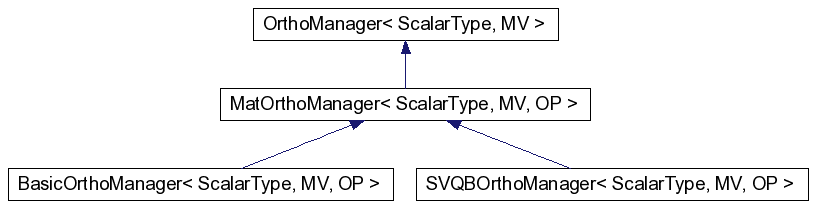
\includegraphics[width=6.0in]{oldhier.png}
\end{center}
\caption{Class inheritance for current framework.}
\label{fig:oldhier}
\end{figure}


\begin{table}[ht]
  \centering
  \caption[Current Ortho. Methods]{This table lists the 
  methods currently provided by the class \textsc{MatOrthoManager}. Note these methods
  differ from those in Table~\ref{tbl:current} by their names and the ability to provide
  the intermediate products needed by the inner product.}
  \begin{tabular}{|c|c|l|}
    \hline \hline
    Inputs                       & Outputs     & Description \\ \hline 

    \multirow{2}{*}{$innerProdMat(S,T,MT)$}         & \multirow{2}{*}{$C$}
    & \multirow{2}{7cm}{Compute inner products $C = S^H M T$} \\
    & & \\\hline

    \multirow{2}{*}{$normMat(S,MS)$}         & \multirow{2}{*}{$z$}
    & \multirow{2}{7cm}{Compute induced norms, $z_i = \sqrt{s_i^H M s_i}$} \\
    & & \\\hline

    \multirow{2}{*}{$normalizeMat(S,MS)$}         & \multirow{2}{*}{$V,B$}
    & \multirow{2}{7cm}{Compute orthonormal $V$ such that $S = V\inner{V}{S} = VB$} \\ 
    & & \\\hline

    $projectMat(Q,S,MS)$         & \multirow{2}{*}{$\hat{S},C$}
    & \multirow{2}{7cm}{Compute $\hat{S}$ such that $\inner{Q}{\hat{S}} = 0$ and $S = \hat{S} + QC$} \\
    $\inner{Q}{Q}=I$ & & \\\hline

    $projectAndNormalizeMat(Q,S,MS)$ & \multirow{2}{*}{$V,C,B$}
    & \multirow{2}{7cm}{Compute orthonormal $V$ such that $\inner{V}{Q}=0$ and $S = QC+VB$} \\
    $\inner{Q}{Q}=I$ & & \\\hline

    \hline
  \end{tabular}
  \label{tbl:currentMat}
\end{table}



A study of these tables reveals some assumptions made by the current framework, both
regarding the form of the input as well as the specific action of the orthogonalization
methods. Some of these assumptions are limiting in our ability to apply some projectors.
Section~\ref{sec:example} describes an example of these limitations.

%%%%%%%%%%%%%%%%%%%%%%%%%%%%%%%%%%%%%%%%%%
\section{Motivating Examples}
\label{sec:example}

%%%%%%%%%
Assume that we wish to apply the projector
\begin{equation}
\Pi = I - M V (V^H M M V)^{-1} V^H M\ ,
\label{eq:piexample}
\end{equation}
where $M$ is a symmetric positive definite matrix. This projector removes the components
of $V$ with respect to the $M$-inner product, via a modification in the range of $MV$.
This projector is used, for example, in a number of optimization-based eigensolvers;
see~\cite{SW82,ST2000,ABG2006-JCAM}.

Only one possibility exists for describing this projector in the current framework. By
setting $\tilde{V} \doteq M V N$, where $N$ is chosen so that $\tilde{V}^H \tilde{V} = N^H
V^H M M V N = I$, we can use the $project()$ method of an \textsc{OrthoManager} employing
the Euclidean inner product:
\[
\hat{S} = project(\tilde{V},S)\ . 
\]
In this way, the resulting multivector satisfies $\inner{\hat{S}}{V}_M = \inner{\hat{S}}{MV}_I =
\inner{\hat{S}}{\tilde{V}N^{-1}}_I = 0$. There are two problems with this approach.

The first problem with this approach is that it required the construction of $\tilde{V}$,
an orthonormal basis for $\range{MV}$. This constraint resulted from the assumption by
$project()$ that the input basis is orthonormal. The construction of this orthonormal
basis can be performed using the orthogonalization manager's $normalize()$ method.
However, it requires additional storage for the multivector $\tilde{V}$, as well as
additional effort on the part of the user.

The second problem with this approach is its reliance on the Euclidean inner product. In
employing the Euclidean inner product for the $project()$ method, the methods
$normalize()$ and $projectAndNormalize()$ will return bases that are orthonormal with
regard to this basis. It is possible for a user requiring $M$-orthonormal bases to employ
the $normalize()$ routine of a second orthogonalization manager, using an $M$-based inner
product. We do not feel that this is a satisfactory solution; it should be possible to
employ a single orthogonalization manager for all needs. Furthermore, the
$projectAndNormalize()$ method (if implemented according to specification) would be
unavailable: orthogonality needs to be defined with respect to the $I$-based inner
product, while normalization needs to be defined according to the $M$-based inner product.


%%%%%%%%%
For another example, consider also the application of the projector 
\begin{equation}
  \Omega = I - K^{-1} M V (V^H M K^{-1} M V)^{-1} V^H M\ ,
  \label{eq:omexample}
\end{equation}
where $M$ is a symmetric positive definite matrix. This projector is used to provide the
solution $T$ to the linear system 
\[
   \Pi K \Pi \, T = U\ ,
\]
where $\Pi$ is as in~\eqref{eq:piexample}, $U = \Pi U$ and we desire $T = \Pi T$. The
solution is given by 
\[
T = (I - K^{-1} M V (V^H M K^{-1} M V)^{-1} V^H M) K^{-1} U\ ,
\]
a formula due to Olsen et al.~\cite{OJS90}. This scenario occurs when preconditioning the
inner iteration for a number of Newton-like eigensolvers;
see~\cite{SW82,SvdV96,ST2000,ABG2006-JCAM}. It is desirable to apply this product via an
orthogonalization routine, as it is often more important that the resultant $T$ is in the
proper subspace than that the system is solved exactly. 

As with Example~\eqref{eq:piexample}, it is possible to finagle the desired solution via
the proper choice of orthogonal projector, inner product and post-application of $K^{-1}$:
\begin{align*}
  U &= K^{-1} U - K^{-1} M V (V^H M K^{-1} M V)^{-1} V^H M K^{-1} U \\
    &= K^{-1} \left( U - \tilde{V} \inner{\tilde{V}}{U}_{K^{-1}} \right) \ ,
\end{align*}
where $\tilde{V}$ is a $K^{-1}$-orthonormal basis for $M V$. This may be an unfavorable
solution, as it requires an orthogonalization manager using the $K^{-1}$-inner product
along with the creation of the temporary basis $\tilde{V}$.


Although these examples employ less common projectors, they illustrates that fact that the
current framework is too strict in dictating the behavior of the $project()$ and
$projectAndNormalize()$ routines. A more general setting will allow us the flexibility to
apply a broader class of projectors.


%%%%%%%%%%%%%%%%%%%%%%%%%%%%%%%%%%%%%%%%%%%%%%
\section{Proposed Framework}
%%%%%%%%%%%%%%%%%%%%%%%%%%%%%%%%%%%%%%%%%%%%%%

We first describe the form of a general projector, in order to design
the proposed framework around this concept. Assume an inner product
$\inner{\cdot}{\cdot}$. Then given bases $X$ and $Y$, define the
general projector as
\[
P_{X,Y} S = S - X \inner{Y}{X}^{-1} \inner{Y}{S}\ .
\]
This projector works by modifying the input in the range of $X$ so that the result is
orthogonal to $Y$. In this way, the projector is specified according to three parameters:
\begin{itemize}
  \item the inner product defining orthogonality, 
  \item a basis $Y$ for the subspace against which the orthogonality is effected, and
  \item a basis $X$ for the subspace where the effect of the projection occurs. 
\end{itemize}
The previous framework allowed only the first two of these three parameters to be
specified. It was assumed there that $X=Y$.

This allows the example from~\eqref{eq:piexample} to be implemented using the
$M$-inner product, by choosing $X=MV$ and $Y=V$:
\[
P_{MV,V} S = S - MV \inner{V}{MV}^{-1}_M \inner{V}{S}_M 
= S - MV (V^H M M V)^{-1} (V^H M S)\ . 
\]
The example from~\eqref{eq:omexample} can be implementing using the $M$-inner product, by
choosing $X=K^{-1} M V$ and $Y=V$, and applying the projector to $K^{-1} U$:
\[
P_{K^{-1} M V, V} K^{-1} U = \left( I - K^{-1} M V \left( V^H M K^{-1} M V \right)^{-1}
V^H M \right) K^{-1} U = T\ .
\]

Therefore, we have the ability to natively manage two of the applications that are not
sufficiently addressed by the current framework.  Furthermore, the current framework is
superseded. The projection operations described there are accessible via the proposed
framework by supplying $X=Y$.  Table~\ref{tbl:proposed} lists the proposed projection
methods, with their abstract definitions. 

One constraint is placed on the inputs $X$ and $Y$. It will be assumed that $\inner{Y}{X}$
is a symmetric positive definite matrix. This has benefit of allowing a Cholesky
factorization to be used in the case that inverse of $\inner{Y}{X}$ needs to be applied.
Note that this requirement does not preclude the application of either example from
Section~\ref{sec:example}.

%%%%%%%%%%%%%%%%%%%%%%%%%%%%%%%%%%%%%%%%%%%%%%%%%%%%%%%%%%%%%%%%%%%%%%%%%%%%%%%%%%%%%%%%%%%%%%%%%%%%%%%%%%%%%%
%%%%%%%%%%%%%%%%%%%%%%%%%%%%%%%%%%%%%%%%%%%%%%%%%%%%%%%%%%%%%%%%%%%%%%%%%%%%%%%%%%%%%%%%%%%%%%%%%%%%%%%%%%%%%%
\begin{table}[ht]
  \centering
  \caption[Proposed Ortho. Methods]{Projection methods under the proposed
  orthogonalization framework.}
  \begin{tabular}{|c|c|p{7cm}|}
    \hline \hline
    Inputs                       & Outputs     & Description \\ \hline 

    $project(X,Y,S)$         & \multirow{2}{*}{$\hat{S},C$}
    & \multirow{2}{7cm}{Compute $\hat{S}$ such that $\inner{Y}{\hat{S}} = 0$ and
    $S = \hat{S} + X C$} \\
    $\inner{Y}{X}$ is s.p.d. & & \\\hline

    $projectAndNormalize(X,Y,S)$ & \multirow{2}{*}{$V,C,B$}
    & \multirow{2}{7cm}{Compute orthonormal $V$ such that $\inner{Y}{V}=0$ and $S =
    XC+VB$} \\ 
    $\inner{Y}{X}$ is s.p.d. & & \\\hline

    \hline
  \end{tabular}
  \label{tbl:proposed}
\end{table}
%%%%%%%%%%%%%%%%%%%%%%%%%%%%%%%%%%%%%%%%%%%%%%%%%%%%%%%%%%%%%%%%%%%%%%%%%%%%%%%%%%%%%%%%%%%%%%%%%%%%%%%%%%%%%%
%%%%%%%%%%%%%%%%%%%%%%%%%%%%%%%%%%%%%%%%%%%%%%%%%%%%%%%%%%%%%%%%%%%%%%%%%%%%%%%%%%%%%%%%%%%%%%%%%%%%%%%%%%%%%%



Recall the desired properties of an orthogonalization framework: 
\begin{enumerate}
  \item[P1.] that it not restrict the efficiency of the orthogonalization routines, either in 
    terms of computational effort or memory requirements;
  \item[P2.] that requirements on the input and output of the orthogonalization routines
    be specified so as to allow their usage without knowing anything about the underlying
    implementation; and 
  \item[P3.] that it be broad enough to enable the implementation of a variety of 
    orthogonalization procedures and techniques.
\end{enumerate}
Table~\ref{tbl:proposed} rigorously describes the orthogonalization methods provided by
the proposed framework, satisfying P2. The generalized projection used in the proposed
framework has more descriptive power than the current framework and enables the
extensibility of the orthogonalization manager, which addresses P3.


The last goal is to ensure that efficient implementation is not hampered by the proposed
framework. One efficiency requirement concerns the application of the general projector:
\[
P_{X,Y} (S) = S - X \inner{Y}{X}^{-1} \inner{Y}{S}\ .
\]
In many cases, the multivectors $X$ and $Y$ may be known to be bi-orthonormal, i.e.,
$\inner{Y}{X} = I$. This is true in particular when $X=Y$ is orthonormal. In this
scenario, we wish to avoid the computation and inversion of $\inner{Y}{X}$, which may
constitute a large portion of the cost of applying the projector, especially as $X$ and
$Y$ grow large relative to $S$. This is not a concern in the current framework, as the
projection operations assume $X=Y$ to be orthonormal. The framework allows for this
consideration by accepting an argument to the $project()$ and $projectAndNormalize()$
methods which specifies the bi-orthogonality of $X$ and $Y$, as shown in
Table~\ref{tbl:proposed_code}.

Note that the proposed framework modifies only the definition of projection; normalization
is not modified. Therefore we need only to expand the methods $project()$ and
$projectAndNormalize()$ to provide this additional capability. The modified interfaces
will be implemented as a new abstract class, \textsc{GenOrthoManager}.  The motivation for
the class \textsc{MatOrthoManager} still stands: in the case of an $M$-based inner
product, we wish to support the provision of $MX$, $MY$ and $MS$.  Therefore,
\textsc{GenOrthoManager} will inherit from \textsc{MatOrthoManager}.  The updated class
hierarchy is listed in Figure~\ref{fig:newhier}.



%%%%%%%%%%%%%%%%%%%%%%%%%%%%%%%%%%%%%%%%%%%%%%%%%%%%%%%%%%%%%%%%%%%%%%%%%%%%%%%%%%%%%%%%%%%%%%%%%%%%%%%%%%%%%%
%%%%%%%%%%%%%%%%%%%%%%%%%%%%%%%%%%%%%%%%%%%%%%%%%%%%%%%%%%%%%%%%%%%%%%%%%%%%%%%%%%%%%%%%%%%%%%%%%%%%%%%%%%%%%%
\begin{argtable}{Proposed GenOrthoManager Class Methods}{This table lists the method signatures for the class
  \textsc{GenOrthoManager}. \texttt{tsdm} is a \textsc{Teuchos::SerialDenseMatrix},
  \texttt{mvec} is a multivector object, and \texttt{bool} is a boolean.}{10cm}{tbl:proposed_code}

  \atmethod{projectGen(X,Y,isBiOrtho,S,C,MX,MY,MS)}
  \atargument{mvec X}{in}{A basis for the subspace where $S$ is modified}
  \atargument{mvec Y}{in}{A basis for the subspace $S$ is projected away from}
  \atargument{bool isBiOrtho}{in}{\texttt{bool} indicating if $\inner{X}{Y}=I$}
  \atargument{mvec S}{in/out}{On output, $\inner{Y}{S_{out}} = 0$ and $S_{in} = S_{out} + XC$}
  \atargument{tsdm C}{out}{The coefficients $C = \inner{X}{Y}^{-1} \inner{Y}{S_{in}}$}
  \atargument{mvec MX}{out}{\textit{Optional:} Provides $M \cdot X$ for the inner product}
  \atargument{mvec MY}{out}{\textit{Optional:} Provides $M \cdot X$ for the inner product}
  \atargument{mvec MS}{out}{\textit{Optional:} On input, provides $M \cdot S_{in}$ for the inner product;  on output, returns $M \cdot S_{out}$}

  \atmethod{projectAndNormalizeGen(X,Y,isBiOrtho,S,C,B,MX,MY,MS)}
  \atargument{mvec X}{in}{A basis for the subspace where $S$ is modified}
  \atargument{mvec Y}{in}{A basis for the subspace $S$ is projected away from}
  \atargument{bool isBiOrtho}{in}{\texttt{bool} indicating if $\inner{X}{Y}=I$}
  \atargument{mvec S}{in/out}{On output, the basis $V$ satisfying $\inner{V}{V}=I$ and $\inner{Y}{V}=0$ and $S_{in} = XC + VB$.}
  \atargument{tsdm C}{out}{The coefficients $C = \inner{X}{Y}^{-1} \inner{Y}{S_{in}}$}
  \atargument{tsdm B}{out}{The coefficients $B = \inner{V}{S_{in}-XC}$}
  \atargument{mvec MX}{out}{\textit{Optional:} Provides $M \cdot X$ for the inner product}
  \atargument{mvec MY}{out}{\textit{Optional:} Provides $M \cdot X$ for the inner product}
  \atargument{mvec MS}{out}{\textit{Optional:} On input, provides $M \cdot S_{in}$ for the inner product;  on output, returns $M \cdot S_{out}$}
  \atargument{return}{}{Returns integer specifying the rank of the computed basis}

\end{argtable}
%%%%%%%%%%%%%%%%%%%%%%%%%%%%%%%%%%%%%%%%%%%%%%%%%%%%%%%%%%%%%%%%%%%%%%%%%%%%%%%%%%%%%%%%%%%%%%%%%%%%%%%%%%%%%%
%%%%%%%%%%%%%%%%%%%%%%%%%%%%%%%%%%%%%%%%%%%%%%%%%%%%%%%%%%%%%%%%%%%%%%%%%%%%%%%%%%%%%%%%%%%%%%%%%%%%%%%%%%%%%%




%%%%%%%%%%%%%%%%%%%%%%%%%%%%%%%%%%%%%%%%%%%%%%%%%%%%%%%%%%%%%%%%%%%%%%%%%%%%%%%%%%%%%%%%%%%%%%%%%%%%%%%%%%%%%%
%%%%%%%%%%%%%%%%%%%%%%%%%%%%%%%%%%%%%%%%%%%%%%%%%%%%%%%%%%%%%%%%%%%%%%%%%%%%%%%%%%%%%%%%%%%%%%%%%%%%%%%%%%%%%%
\begin{figure}[ht]
\begin{center}
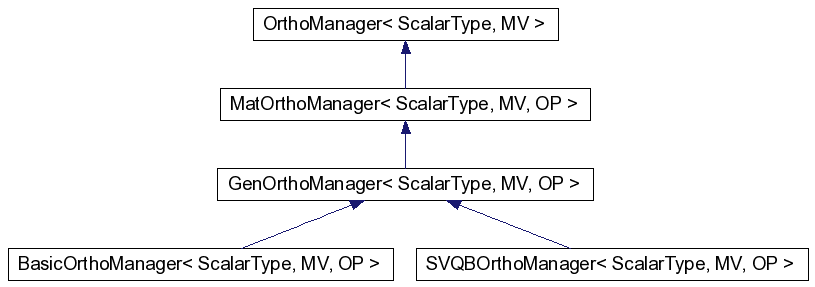
\includegraphics[width=6.0in]{newhier.png}
\end{center}
\caption{Class inheritance for proposed framework.}
\label{fig:newhier}
\end{figure}
%%%%%%%%%%%%%%%%%%%%%%%%%%%%%%%%%%%%%%%%%%%%%%%%%%%%%%%%%%%%%%%%%%%%%%%%%%%%%%%%%%%%%%%%%%%%%%%%%%%%%%%%%%%%%%
%%%%%%%%%%%%%%%%%%%%%%%%%%%%%%%%%%%%%%%%%%%%%%%%%%%%%%%%%%%%%%%%%%%%%%%%%%%%%%%%%%%%%%%%%%%%%%%%%%%%%%%%%%%%%%



%%%%%%%%%%%%%%%%%%%%%%%%%%%%%%%%%%%%%%%%%%%%%%
\section{Transition and Testing}
%%%%%%%%%%%%%%%%%%%%%%%%%%%%%%%%%%%%%%%%%%%%%%

The proposed changes to the framework can be implemented so as to enable easy testing and
avoid any conflict with existing code. Because \textsc{GenOrthoManager} extends the
current framework by inheriting from the lowest level of the orthogonalization manager
class hierarchy, no changes are necessary for the existing classes. The new projection
methods can be implemented alongside the current implementations. Existing code using the
interfaces \textsc{OrthoManager} and \textsc{MatOrthoManager} would be linked with the
current and proven implementations. Furthermore, as the proposed methods
$projectGen()$ and $projectAndNormalizeGen()$ generalize the methods $projectMat()$ and
$projectAndNormalizeMat()$, a class which retains the previous implementations of these
methods has a trivial means by which to validate a subset of the functionality of
the new implementations.

For this reason, the transition from the current to the proposed framework would include
moving the concrete orthogonalization managers \textsc{BasicOrthManager} and
\textsc{SVQBOrthoManager} underneath \textsc{GenOrthoManager}. The existing
implementations supporting \textsc{MatOrthoManager} and \textsc{OrthoManager} can remain
as they are for an initial testing period, while new implementations can be created to
support the projection methods of \textsc{GenOrthoManager}.

% ---------------------------------------------------------------------- %
% References
%
\clearpage
% If hyperref is included, then \phantomsection is already defined.
% If not, we need to define it.
\providecommand*{\phantomsection}{}
\phantomsection
\addcontentsline{toc}{section}{References}
\bibliographystyle{plain}
\bibliography{OrthoStudy}



%
% This is an example of how to create the distribution page. Some
% distributions are required by Sandia; e.g. the housekeeping copies.
% Depending on the type of report; e.g. CRADA, Patent Caution, etc.
% additional distribution lines may have to be added. See the
% "Guide for Preparing SAND Reports"
%
% SANDdistribution takes CA or NM as an optional argument. If given,
% the approrpiate housekeeping copies are inserted autmatically.
% Inside the SANDdistribution environment, several commands can be used
% insert the distributions for CRADA, LDRD, etc. See example below.
%
% You can leave the CA or NM option off and not use any of the SANDdist*
% commands. This will allow you to create a distribution list manually.
%
\begin{SANDdistribution}[NM]
    % Housekeeping copies necessary for every unclassified report:
    % \SANDdistCRADA	% If this report is about CRADA work
    % \SANDdistPatent	% If this report has a Patent Caution or Patent Interest
    % \SANDdistLDRD	% If this report is about LDRD work

    % Some external Addresses

    \SANDdistExternal{1}{Roscoe A. Bartlett\\ Oak Ridge National Laboratory \\ P.O. Box 2008 \\ Oak Ridge, Tennessee 37831 \\ United States }
    % \SANDdistExternal{3}{Some Address\\ and street\\City, State}
    % \SANDdistExternal{12}{Another Address\\ On a street\\City, State\\U.S.A.}
    %\bigskip

    % The following MUST BE between the external and internal distributions!
    % \SANDdistClassified % If this report is classified

    % Internal Addresses
    \SANDdistInternal{1}{9018}{Central Technical Files}{8945-1}
    \SANDdistInternal{2}{0899}{Technical Library}{9610}
    \SANDdistInternal{2}{0612}{Review \& Approval Desk}{4916}
    \SANDdistInternal{1}{0897}{Todd S. Coffey}{1543}
    \SANDdistInternal{1}{1320}{Curtis C. Ober}{1442}
    \SANDdistInternal{1}{1318}{Roger P. Pawlowski}{1444}
    
    % Example of a mail channel use (instead of a mail stop)
    % \SANDdistInternalM{1}{M9999}{Someone}{01234}

\end{SANDdistribution}


\end{document}
